\documentclass[12pt]{article}
\usepackage[utf8]{inputenc}
\usepackage[english]{babel}
\usepackage{amsmath}
\usepackage{amssymb}
\usepackage{bm}
\usepackage{listings}
\usepackage{minted}
\usepackage{graphicx}
\usepackage{subfig}

\graphicspath{./images/}
\setlength\parindent{0pt} % Removes all indentation from paragraphs
\newcommand{\uvec}[1]{\boldsymbol{\hat{\textbf{#1}}}}
\title{ECE421 - Winter 2021 \\ Unsupervised Learning and Probabilistic Models}
\author{Shayshu Nahata-Ragubance}
\date{\today}
\begin{document}
\maketitle

\section{Objectives}
Implement learning and inference procedures for K-means, and GMM. 

\section{K-means}
\subsection{Learning K-means}
Shown below is the implementation of the distance function, and the training code
for the K-means algorithm,  as well as the results from training the model
on the data2D.npy dataset.

\begin{minted}{Python}
# Distance function for K-means
def distanceFunc(X, MU):
  # Inputs
  # X: is an NxD matrix (N observations and D dimensions)
  # MU: is an KxD matrix (K means and D dimensions)
  # Outputs
  # pair_dist: is the pairwise distance matrix (NxK)

  X_expand = tf.expand_dims(X, 0)
  MU_expand = tf.expand_dims(MU, 1)

  sqr_distance = tf.square(tf.subtract(X_expand, MU_expand))
  sqr_distance = tf.reduce_sum(sqr_distance, axis = 2)
  sqr_distance = tf.transpose(sqr_distance)

  return sqr_distance
\end{minted}

\begin{minted}{Python}
def buildGraphKM(data, data_dim, K, lr):
  data_points = tf.placeholder(tf.float32, (None, data_dim), \
      name = "data")

  # Initialize the cluster centers based on a random sample of
  # data points in the set...
  centers = tf.Variable(tf.cast(tf.slice(tf.random_shuffle(data), \
      [0, 0], (K, -1)), dtype=tf.float32), dtype=tf.float32)

  # Out loss function is the pairwise distance between points and 
  # their cluster centers...
  loss = tf.reduce_sum(tf.reduce_min(distanceFunc(data_points, centers), \ 
      axis = 1))

  optim = tf.train.AdamOptimizer(learning_rate=lr, beta1=0.9, \ 
      beta2=0.99, epsilon=1e-5)
  optim = optim.minimize(loss)

  return data_points, centers, optim, loss
\end{minted}

\begin{minted}{Python}
def plotScatter(title, sample_points, centers, K, size, \
  assign, min_val_loss):
  
  frequency = np.bincount(assign)
  index = np.nonzero(frequency)[0]
  frequency = zip(index, frequency[index])

  iter = 1
  percentages = []
  for i in frequency:
    percentages.append("Cluster " + str(i[0] + 1) + " " + \
      str(round((i[1] / len(assign)) * 100, 2)) +  "%")
    iter += 1

  plt.title(title)
  
  for i in range(K):
    plt.scatter(sample_points[i][:, 0], sample_points[i][:, 1], \
      alpha=1, s=5, label = percentages[i])

  plt.scatter(centers[:, 0], centers[:, 1], marker='x', \
      s = 50, c='black')

  plt.text(0, -6.5, "Validation loss: " + str(min_val_loss), \
      ha='center')

  plt.legend()
  plt.show()
  return
\end{minted}

\begin{minted}{Python}
def sampleColours(sample_points, centers):
  # For each sample find the closest center 
  # and then assign it a colour...
  closest = tf.arg_min(distanceFunc(sample_points, centers), 1)
  return closest
\end{minted}

\begin{minted}{Python}
def K_means(K, lr, is_valid = False, epochs=10, plot=True, npy=2):
  train_loss = []
  val_loss = []

  # Loading data
  if (npy == 2):
    data = np.load('data2D.npy')
  else:
    data = np.load('data100D.npy')
  [num_pts, dim] = np.shape(data)

  # For Validation set
  if is_valid:
    valid_batch = int(num_pts / 3.0)
    np.random.seed(45689)
    rnd_idx = np.arange(num_pts)
    np.random.shuffle(rnd_idx)
    val_data = data[rnd_idx[:valid_batch]]
    data = data[rnd_idx[valid_batch:]]
  
  X, MU, optim, loss = buildGraphKM(data, dim, K, lr)

  init_op = tf.global_variables_initializer()
  tf.set_random_seed(1000)

  with tf.Session() as sess:
    sess.run(init_op)
    print("Starting K-means...")

    feed = {
      X : data
    }

    for itteration in range(epochs):
      centers, losses, _ = sess.run([MU, loss, optim], \
          feed_dict = feed)

      train_loss.append(losses / len(data))

      # Calculate the validation loss
      if is_valid:
        valid_center, valid_loss, _ = sess.run([MU, loss, optim], \ 
          feed_dict  = {X : val_data})
        val_loss.append(valid_loss / len(val_data))


    colours = sess.run(sampleColours(data, centers), \
      feed_dict = {X: data, MU : centers})
  
  cluster_data = []

  for i in range(K):
    cluster_data.append(data[colours == i])

  if (plot):
    min_loss = round(val_loss[np.argmin(val_loss)], 4)

    plotScatter("K-means Clustering", cluster_data, \ 
      centers, K, len(data), colours, min_loss)

  plt.title("K-means loss")
  plt.plot(train_loss, label="Training loss")
  plt.plot(val_loss, label="Validation loss")
  plt.legend()
  plt.show()
  return train_loss, val_loss
\end{minted}

\begin{flushleft}
    After reviewing the graphs shown below, the best number of clusters to use is 
    5 because all the centers are properly spaced from one another, the data points whitin 
    a cluster do not lie far from the centers unlike the clustering seen in K = 3, for example.
    On top of this the centers seem to be located in areas of high density, indicating that they 
    are representative of a given cluster.
    To confirm this, if the validation loss is checked it shows that using 5 clusters yields the 
    lowest loss.
\end{flushleft}

\begin{figure}[h]
    \centering 
    \subfloat{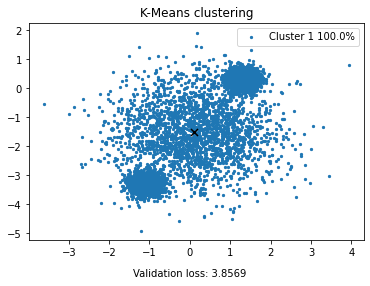
\includegraphics[scale=0.5] {images/km1_scatter.png}}
    \hfill
    \subfloat{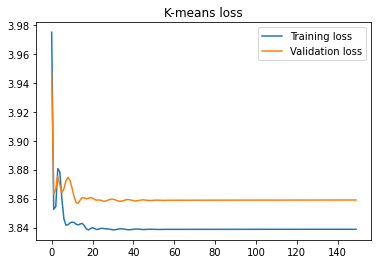
\includegraphics[scale=0.5] {images/km1_loss.png}}
    \caption{K = 1}
\end{figure}

\begin{figure}[!tbp]
    \centering
    \subfloat{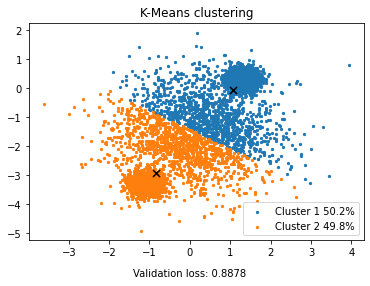
\includegraphics[scale=0.5] {images/km2_scatter.png}}
    \hfill
    \subfloat{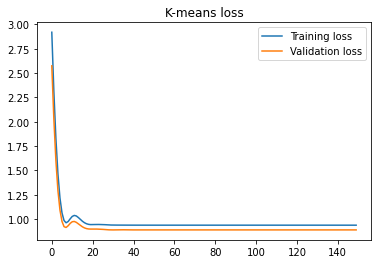
\includegraphics[scale=0.5] {images/km2_loss.png}}
    \caption{K = 2}
\end{figure}

\begin{figure}[!tbp]
    \centering
    \subfloat{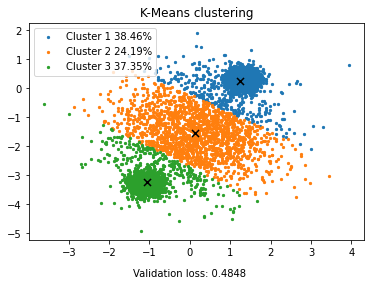
\includegraphics[scale=0.5] {images/km3_scatter.png}}
    \hfill
    \subfloat{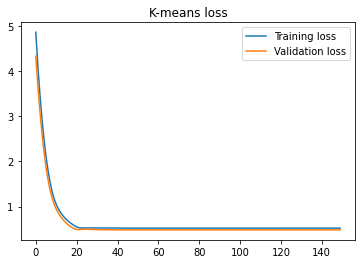
\includegraphics[scale=0.5] {images/km3_loss.png}}
    \caption{K = 3}
\end{figure}

\begin{figure}[!tbp]
    \centering
    \subfloat{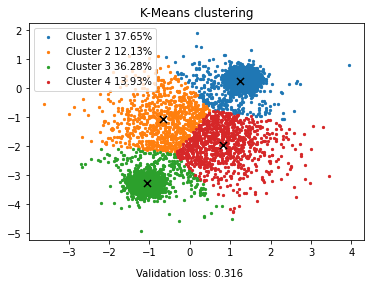
\includegraphics[scale=0.5] {images/km4_scatter.png}}
    \hfill
    \subfloat{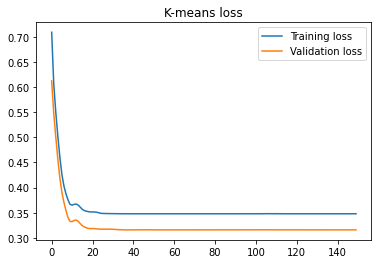
\includegraphics[scale=0.5] {images/km4_loss.png}}
    \caption{K = 4}
\end{figure}

\begin{figure}[h]
    \centering
    \subfloat{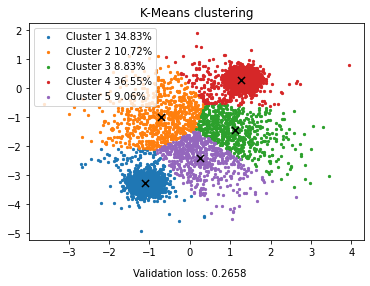
\includegraphics[scale=0.5] {images/km5_scatter.png}}
    \hfill
    \subfloat{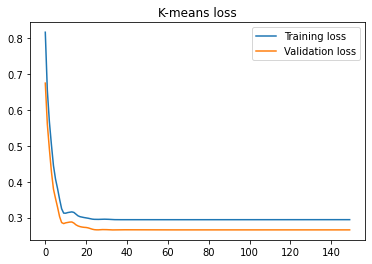
\includegraphics[scale=0.5] {images/km5_loss.png}}
    \caption{K = 5}
\end{figure}

\newpage
\subsection{The Gaussian cluster model}
Shown below is the code used to calculate the logarithm of the Gaussian PDF, as well as
the condtion log probability of clusters given a data point:

\begin{minted}{Python}
def log_GaussPDF(X, mu, sigma):
  # Inputs
  # X: N X D
  # mu: K X D
  # sigma: K X 1

  # Outputs:
  # log Gaussian PDF N X K

  # Recall pdf of gaussian:
  # pdf(x; mu, sigma) = exp(-0.5 (x - mu)**2 / sigma**2) / Z
  # Z = (2 pi sigma**2)**0.5
  # log(pdf) = (-0.5 (x - mu)**2 / sigma ** 2) - log(Z)

  data_dim = tf.cast(X.shape[1], tf.float32)
  Z = (2 * np.pi * tf.square(sigma))
  Z = (data_dim/2) * tf.log(Z)
  pdf = -0.5 * tf.divide(distanceFunc(X, mu), \
      tf.squeeze(tf.square(sigma)))

  log_gauss = pdf - tf.transpose(Z)
  return log_gauss
\end{minted}

\begin{minted}{Python}
def log_posterior(log_PDF, log_pi):
  # Input
  # log_PDF: log Gaussian PDF N X K
  # log_pi: K X 1

  # Outputs
  # log_post: N X K

  # log[P(z | x)] = log[P(x | z)] + log[P(z)] - 
  #                 log[Sum_1_N{exp(log[P(x | z)] + log[P(z)])}] 

  log_post_num = tf.add(log_PDF, tf.transpose(log_pi)) 
  log_post_dem = reduce_logsumexp(log_PDF + log_pi, keep_dims=True)

  return log_post_num - log_post_dem
\end{minted}

\subsection{Learning the MoG} 
Shown below is the code the distance function, a log Gaussian function, a posterior function, 
and a computational graph function, in that code shows
the loss function used and the clustering assignment as well as the optimizer. 
Also shown below is the training code used to train the model.

\begin{minted}{Python}
def buildGraphGMM(data, data_dim, K, lr, div):
  data_points = tf.placeholder(tf.float32, (None, data_dim), \ 
      name = "data")

  # Initialize the cluster centers based on a random sample of
  # data points in the set..
  centers = tf.Variable(tf.cast(tf.slice(tf.random_shuffle(data), \ 
  [0, 0], (K, -1)), dtype=tf.float32), dtype=tf.float32) 

  # Initialize the standard deviation of each function 
  # to be a random sample from a gaussian distribution
  # Make it exponential to deal with constraint...
  sigma = tf.Variable(tf.random_normal((K, 1), stddev= div), \
      dtype=tf.float32)
  sigma = tf.exp(sigma)

  # The weights of each distribution 
  # But again because we're using exp sigma, we need to change 
  # pi_k to be represented by a softmax function
  pi = tf.Variable(tf.random_normal((K, 1), stddev= div), \
      dtype=tf.float32)
  pi = tf.squeeze(logsoftmax(pi))
  
  # Loss = -log[P(X)] 
  #      = -log[[pi_1_N{P(x_n)}]
  #      = -log[Pi_1_N{Sum_1_K{Pi_k N(x_n)}}]
  #      = -log[Pi_1_N{Sum_1_K{e ^ (log[Pi_k] + log[N(x_n)])}}]
  #      = -log[Pi_1_K{e ^ (log[Pi_k] + log[N(x_1)])}] - ... 
  #        -log[Pi_1_K{e ^ (log[Pi_k] + log[N(x_N)])}]
  log_pdf = log_GaussPDF(data_points, centers, sigma)
  loss = reduce_logsumexp(log_pdf + pi, 1, keep_dims=True)
  loss = -1 * tf.reduce_sum(loss)

  optim = tf.train.AdamOptimizer(learning_rate=lr, \ 
      beta1=0.9, beta2=0.99, epsilon=1e-5)
  optim = optim.minimize(loss)

  # Based on the distributions make a prediction as to which 
  # cluster a data point belongs too
  classify = log_posterior(log_pdf, pi)
  classify = tf.nn.softmax(classify)
  classify = tf.argmax(classify, axis = 1)

  return data_points, centers, sigma, pi, optim, loss, classify
\end{minted}

\begin{minted}{Python}
def GMM(K, lr, stddve, is_valid = False, epochs=10, plot=True, npy=1):
  train_loss = []
  val_loss = []
  train_cluster = []

  # Loading data
  if (npy == 2):
    data = np.load('data2D.npy')
  else:
    data = np.load('data100D.npy')
  
  [num_pts, dim] = np.shape(data)

  # For Validation set
  if is_valid:
    valid_batch = int(num_pts / 3.0)
    np.random.seed(45689)
    rnd_idx = np.arange(num_pts)
    np.random.shuffle(rnd_idx)
    val_data = data[rnd_idx[:valid_batch]]
    data = data[rnd_idx[valid_batch:]]
  
  X, MU, sigma, pi, optim, loss, classify = \
      buildGraphGMM(data, dim, K, lr, stddve)

  init_op = tf.global_variables_initializer()
  tf.set_random_seed(1000)

  with tf.Session() as sess:
    sess.run(init_op)
    print("Starting GMM...")

    feed = {
      X : data
    }

    for itteration in range(epochs):
      centers, losses, cluster_assign, _ = \
          sess.run([MU, loss, classify, optim], \
          feed_dict = feed)

      train_loss.append(losses / len(data))
      train_cluster.append(cluster_assign)

      if is_valid:
        valid_center, valid_loss, _c, _o = \
          sess.run([MU, loss, classify, optim], \
          feed_dict = {X : val_data})
        val_loss.append(valid_loss / len(val_data))
    
    # Create scatter plot
    cluster_data = []
    
    for i in range(K):
      cluster_data.append(data[cluster_assign == i])

  if (plot):  
    min_loss = round(val_loss[np.argmin(val_loss)], 4)

    plotScatter("GMM Clustering", cluster_data, centers, K, \ 
      len(data), cluster_assign, min_loss)

  plt.title("GMM loss")
  plt.plot(train_loss, label="Training loss")
  plt.plot(val_loss, label="Validation loss")
  plt.legend()
  plt.show()

  return train_loss, val_loss
\end{minted}

Shown below are the scatter plots and loss graphs for running GMM on the data2D.npy
dataset. Furthermore, the trained parameters for K = 3 are shown below:

\begin{center}
  \begin{table}[h]
    \centering
    \begin{tabular}{|| c c c ||}
      \hline
      $\sigma$ : & 0.9934453& 0.1977245\\
      \hline
    \end{tabular}
  \end{table}
\end{center}

\begin{center}
  \begin{table}[h]
    \centering
    \begin{tabular}{|| c c c c ||}
      \hline
      $\pi$ :& -1.094792& -1.1026771& -1.0983831\\
      \hline
    \end{tabular}
  \end{table}
\end{center}

\begin{center}
  \begin{table}[h]
    \centering
    \begin{tabular}{|| c c c c ||}
      \hline
      $\mu$ :& (0.10631, -1.5272)& (-1.1020, -3.306)& (1.2982, 0.30938)\\
      \hline
    \end{tabular}
  \end{table}
\end{center}

\begin{figure}[h]
    \centering 
    \subfloat{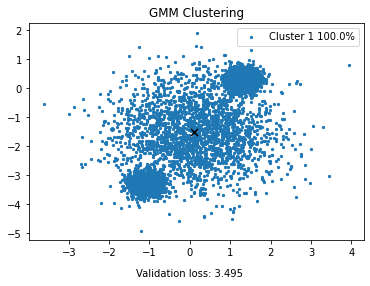
\includegraphics[scale=0.5] {images/gm1_scatter.png}}
    \hfill
    \subfloat{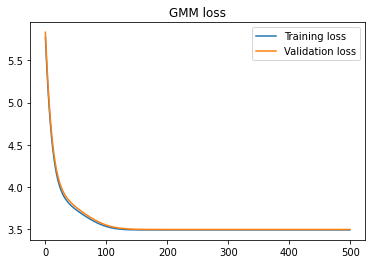
\includegraphics[scale=0.5] {images/gm1_loss.png}}
    \caption{K = 1}
\end{figure}

\begin{figure}[h]
    \centering
    \subfloat{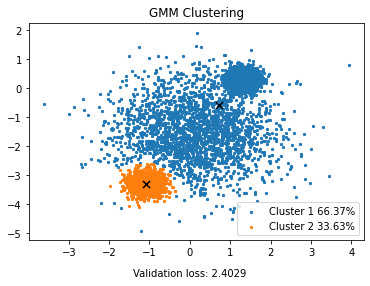
\includegraphics[scale=0.5] {images/gm2_scatter.png}}
    \hfill
    \subfloat{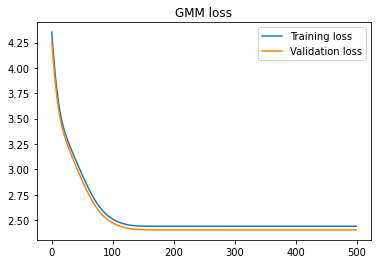
\includegraphics[scale=0.5] {images/gm2_loss.png}}
    \caption{K = 2}
\end{figure}

\begin{figure}[h]
    \centering
    \subfloat{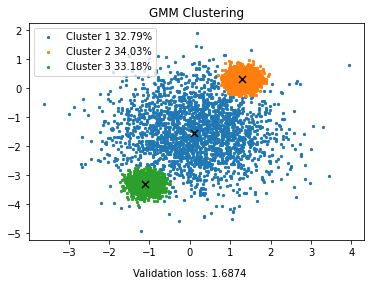
\includegraphics[scale=0.5] {images/gm3_scatter.png}}
    \hfill
    \subfloat{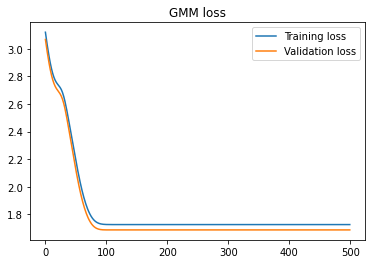
\includegraphics[scale=0.5] {images/gm3_loss.png}}
    \caption{K = 3}
\end{figure}

\begin{figure}[h]
    \centering
    \subfloat{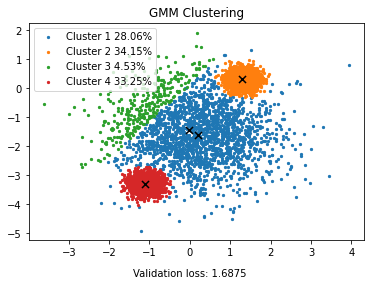
\includegraphics[scale=0.5] {images/gm4_scatter.png}}
    \hfill
    \subfloat{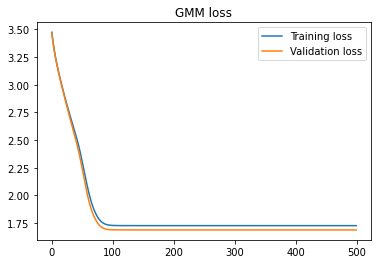
\includegraphics[scale=0.5] {images/gm4_loss.png}}
    \caption{K = 4}
\end{figure}

\begin{figure}[!tbp]
    \centering
    \subfloat{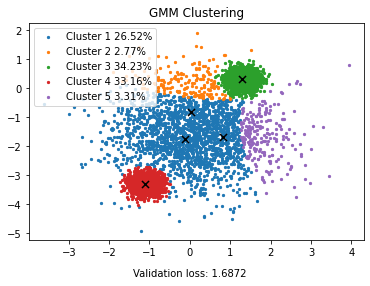
\includegraphics[scale=0.5] {images/gm5_scatter.png}}
    \hfill
    \subfloat{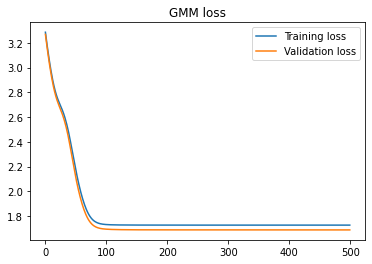
\includegraphics[scale=0.5] {images/gm5_loss.png}}
    \caption{K = 5}
\end{figure}

\newpage
\newpage
Based off of the validation loss the best number of clusters is 5, because it
had the lowest loss at 1.6872. However, the validation loss with 3 and 4 clusters was 1.6974, and 
1.6975 respectively. So, althrough 5 clusters is the best option, 3 clusters will work basically 
just as well. \\

Shown below is the validation loss for running K-Means and GMM on the data100D.npy
dataset:

\begin{center}
  \begin{table}[h]
    \centering
    Number of clusters \\
    \begin{tabular}{||c c c c c||}
      \hline
      5 & 10 & 15 & 20 & 30 \\
      \hline \hline 
      85.469& 48.517& 48.2864& 47.978& 47.876\\
      \hline
    \end{tabular}
    \caption{Validation loss for K-means}
  \end{table}
\end{center}

\begin{center}
  \begin{table}[h]
    \centering
    Number of clusters \\
    \begin{tabular}{||c c c c c||}
      \hline
      5 & 10 & 15 & 20 & 30 \\
      \hline \hline 
      21.659& 20.872& 20.534& 20.391& 20.010 \\
      \hline
    \end{tabular}
    \caption{Validation loss for GMM}
  \end{table}
\end{center}

Plotting these losses again the number of clusters yeilds the following graphs:

\begin{figure}[!tbp]
  \centering
  \subfloat{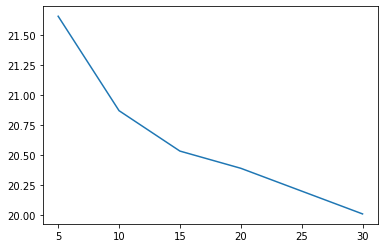
\includegraphics[scale=0.5] {images/km_lossvk.png}}
  \hfill
  \subfloat{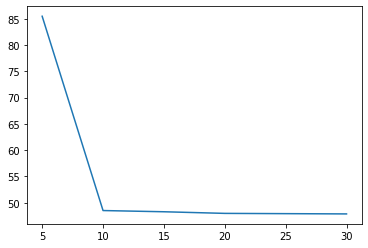
\includegraphics[scale=0.5] {images/gmm_lossvk.png}}
  \caption{Validation loss versus number of clusters. K-means left, GMM right}
\end{figure}

\newpage
Based off this, it can be concluded that the dataset has at least 3 clusters. This is 
shown because in the GMM loss versus cluster graph the loss converges at K = 10. However, 
the K-means loss versus cluster graph does not seem to converge at K = 10, but the 
slope of the graph decreases after K = 10. So using this knowledge as bounds, the dataset
has at least 10 clusters.  
\end{document}